\documentclass[draftcls,onecolumn]{IEEEtran}

%% INCLUDING THE PREAMBLE
%%%%%%%%%%%%%%%%%%%%%%%%%%%%%%%%%%%%%%%%%%%%%%%%%%%%%%%%%%%%%%%%%%%%%%%%%%%
%                                                                         %
%                                 PREAMBLE                                %
%                                                                         %
%%%%%%%%%%%%%%%%%%%%%%%%%%%%%%%%%%%%%%%%%%%%%%%%%%%%%%%%%%%%%%%%%%%%%%%%%%%

%% PACKAGES
\usepackage[]{lineno}
%\linenumbers
\usepackage[usenames,dvipsnames]{xcolor}
\usepackage{microtype}
\usepackage[obeyDraft]{todonotes}
\usepackage{fancyvrb}
\VerbatimFootnotes
\usepackage{algorithmic}

%% GRAPHICS RELATED
\usepackage{graphicx}
\usepackage[outdir=./tmp/]{epstopdf}
\graphicspath{{../images/}{./}{./tmp/}}
\DeclareGraphicsExtensions{.eps, .pdf, .jpeg, .png,}

%% CPATION SETUP
\usepackage{float}
\usepackage{caption}
\usepackage{subcaption}
\captionsetup{belowskip=12pt,aboveskip=4pt}


%% BIBLIOGRAPHY
\bibliographystyle{ieeetr}

%% UNITS
\usepackage{siunitx}

%% EQUATIONS
\usepackage{amsmath}
%\numberwithin{equation}{section}

%% HYPERLINKS
\usepackage[debug]{hyperref}

%%%%%%%%%%%%%%%%%%%%%%%%%%%%%%%%%%%%%%%%%%%%%%%%%%%%%%%%%%%%%%%%%%%%%%%%%%%
%                                                                         %
%                             Listing Setup                               %
%                                                                         %
%%%%%%%%%%%%%%%%%%%%%%%%%%%%%%%%%%%%%%%%%%%%%%%%%%%%%%%%%%%%%%%%%%%%%%%%%%%
\usepackage{listings}
\lstset{ %
    language=C++,
    basicstyle=\footnotesize\ttfamily,
    numbers=left,
    numberstyle=\tiny\color{gray},
    stepnumber=2,
    numbersep=5pt,
    backgroundcolor=\color{white},
    showspaces=false,
    showstringspaces=false,
    showtabs=false,
    frame=single,
    rulecolor=\color{black},
    tabsize=2,
    breaklines=true,
    breakatwhitespace=false,
    title=\lstname,
    keywordstyle=\color{blue},
    commentstyle=\color{OliveGreen},
    stringstyle=\color{orange}
}
\DeclareCaptionFont{white}{\color{white}}
\DeclareCaptionFormat{listing}{\colorbox[cmyk]{0.43, 0.35, 0.35, 0.01}{\parbox{\dimexpr\textwidth-2\fboxsep\relax}{#1#2#3}}}
\captionsetup[lstlisting]{format=listing,labelfont=white,textfont=white,singlelinecheck=false,margin=0pt,font={bf,footnotesize}}
%\lstnewenvironment{code}[1][]%
%{ \noindent\minipage{\linewidth}
%	\lstset{#1}
%}
%{\endminipage}
%% USER COMMANDS
\usepackage{isotope}
\newcommand{\iso}{\isotope}
\newcommand{\figurewidth}{\textwidth}
\newcommand{\micron}{$\mu$m}



%%%%%%%%%%%%%%%%%%%%%%%%%%%%%%%%%%%%%%%%%%%%%%%%%%%%%%%%%%%%%%%%%%%%%%%%%%%
%                                                                         %
%                                Start of Document                        %
%                                                                         %
%%%%%%%%%%%%%%%%%%%%%%%%%%%%%%%%%%%%%%%%%%%%%%%%%%%%%%%%%%%%%%%%%%%%%%%%%%%
\begin{document}
\title{Comparison of Lithated Glass, LiF:ZnS(Ag), Boron Loaded Pastic, and PEN Films}
\author{Matthew J. Urffer}
\date{\today}
\maketitle

% Tables of Contents, Figures, Tables
\tableofcontents
\listoffigures
\listoftables
%%%%%%%%%%%%%%%%%%%%%%%%%%%%%%%%%%%%%%%%%%%%%%%%%%%%%%%%%%%%%%%%%%%%%%%%%%%
%                                                                         %
%                              Start of Content                           %
%                                                                         %
%%%%%%%%%%%%%%%%%%%%%%%%%%%%%%%%%%%%%%%%%%%%%%%%%%%%%%%%%%%%%%%%%%%%%%%%%%%
\section{Introduction}

\subsection{Previous Work}

Work by Guerard (published slides) has published slides of the performance of GS20 and a LiF:ZnS film (\autoref{fig:GuerardLightYield}).
It should be noted for the start that Guerard's measurment is not the same as ours - the neutron source is unkown, as well is the suplier of the LiF:ZnS film (and thickness). 
In addition, the thicknes of GS20 reported by Guerard is \SI{0.5}{\mm} while the GS20 in the detection lab is \SI{2}{\mm}.
\begin{figure}
  \centering
  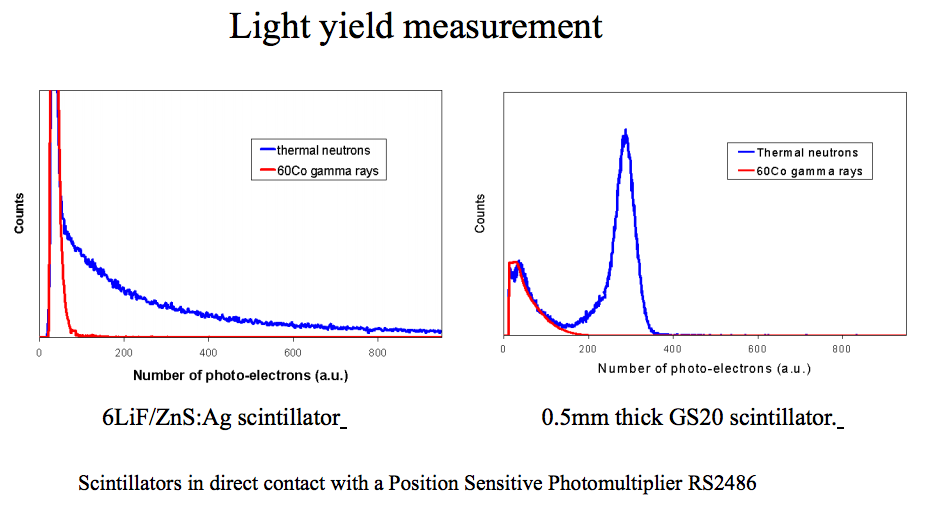
\includegraphics[width=\textwidth]{Guerard_LightYieldMeasurement.tiff}
  \caption[Measured Light Yield (Guerard)]{Light yeild as measured by Guerard. The GS20 measurement has a lower gamma performance than as measured, and the LiF:ZnS does not have the same shape as we measured}
	\label{fig:GuerardLightYield}
\end{figure}
The following figure, \autoref{fig:GuerardIntEff}, shows the neutron detection efficiency and sensitivity to \iso[60]{Co} rays.
For a senisitivity of \num{10E-6} the LiF:ZnS film is reported to have a neutron detection efficiency of 60\%, while the \SI{1}{\mm} GS20 has a reported neutron detection efficiency of 55\%.
\begin{figure}
  \centering
  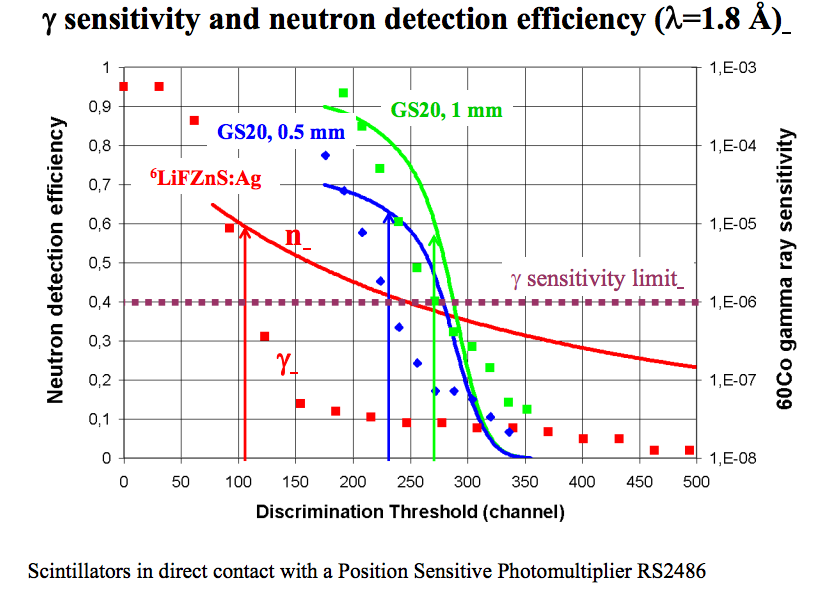
\includegraphics[width=\textwidth]{Guerard_IntEff_NCr.tiff}
  \caption[Intrisinic Efficiency (Geurard)]{Intrisinic Efficiency of LiF:ZnS and GS20 from Guerard.  The gamma intrisinic efficiency is shown in the solid squares (right axis), while the lines show the nuetron efficiency (left axis). The values reported here are much higher than the values reported in this report.}
	\label{fig:GuerardIntEff}
\end{figure}

\section{Methods}

\subsection{Mass of \iso[6]{Li} in Samples}
The mass of \iso[6]{Li} was cacluated for each of the sample in order to normalize the samples performance.
\begin{align}

\end{align}

The quantaum efficiency of the PMT is expected to decrease at lower voltages.
Thus, measuring the films using a low voltage to power the PMT (necessary in order to measure the high light yield of the LiF:ZnS) might cause the film performance to be lower than measuring it at a more optimal voltage.


\section{Results}

\subsection{Agreement to Previous Results}
It is observed from \autoref{fig:GuerardIntEff} that the neutron spectra has the same endpoint while the gamma sensitivity increases with thickness.
Assuming a linear increase in the gamma sensitity with thickness, a \SI{2}{\mm} would then be expected 

\section{Conclusions}

\end{document}
